%%%%%%%%%%%%
%% Om Mig %%
%%%%%%%%%%%%

\Section
{Om Mig}
{Om Mig}
{PDF:OmMig}
Asger, 23 år.

\begin{minipage}{0.6\textwidth}% adapt widths of minipages to your needs
Jeg er oprindeligt fra Nordsjælland, Hornbæk, men flyttede til Aalborg i 2015 sammen med min kæreste, idet vi begge skulle studere på Aalborg Universitet.
Jeg er nu blevet Bachelor i Datalogi, og søger et spændende og udfordrende job, hvor jeg kan anvende min nuværende viden og opbygge nye relevante kompetencer. Jeg har indtil videre erfaring med Python, C\#, ANSI C, BASH, Linux og en smule Assembly, Windows og C++.

Eftersom Aalborg Universitet er meget virksomhedsnær, som følge af deres model med problembaseret læring (PBL), har jeg i hvert semester arbejdet med projekter. Disse projekter har givet mig erfaring med at arbejde i teams af op imod syv personer, med varierende grad af samarbejde og individuelt arbejde, hvor vi har anvendt alt fra iterative til sekventielle teknikker igennem systemudvikling. På baggrund heraf vil jeg egne mig godt til at arbejde i teams, hvad enten de er præget af nært teamwork eller individuelle bidrag til et fælles projekt.
\end{minipage}%
\hfill
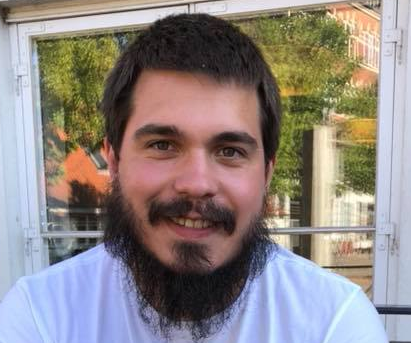
\includegraphics[]{Images/ProfilBilled.png}
